\chapter{Specification} % (fold)
\label{cha:specification}

\section{Introduction}
In this phase we made the specification of the game. The description in the assignment has been kept quite vague by the OGO-organisation and in this phase we have made it much more detailed. First we had a brainstorm session, generating a number of possible variations. Then we chose one of these variations and selected features, organising those features by feasibility and attractiveness, using the MOSCoW method, as mentioned in the orientation document (``werkdocument''). In this part, we describe these choices.

\section{The assignment}
This is the assignment, as described in the ``projectwijzer'':

`Gevraagd wordt om een interactief, gedistribueerd 3D spel te
ontwikkelen. Gedistribueerd houdt hier in dat iedere speler zijn eigen
beeldscherm gebruikt en dat alle schermen een weergave van dezelfde
spelsituatie tonen. Op het speelveld bevinden zich twee tot zes spelers.
Verder is verspreid over het speelveld ``voedsel'' aanwezig. Doel van het
spel is zo veel mogelijk voedsel te verzamelen. Wat zich verder op het
speelveld bevindt wordt aan de ontwikkelaars overgelaten. Belangrijk is
dat het spel leuk is om te spelen, er attractief uitziet en natuurlijk nooit
faalt.'

\section{Definitions} % (fold)
\label{sec:definitions}
Table \ref{table:definitions} has some definitions of terms used in this document.

\begin{table}[h!t!]

    \begin{tabular}{l|l}
        \hline
        \hline
        Term                & Explanation \\
        \hline
        \hline
        Bomb3D              & The name of the game. We usually mean the application itself. \\
        \hline
        Game                & An instance of Bomb3D, currently running in a match. \\ 
        \hline
        Avatar              & A 3D model, representing the player in the game (we will use word player mostly throughout this document) \\
        \hline
        Continuous Movement & More or less fluid movement; the player does not stick to a grid or \\
                            & take discrete steps \\
        \hline
        First Person        & The player views the game from the eyes of his avatar \\
        \hline
        Level               & A model of a maze-like 3d-environment, described by a map \\
        \hline
        Mini map            & A small map of the level on the edge of the screen \\
        \hline
        Power-up            & An item, represented by a model in-game, that can be picked up by an \\
                            & avatar and give him or her some bonus or extra power, hence the name \\
        \hline
        Spawn               & Being placed in the level \\
        \hline
        Soft wall           & A soft wall can be destroyed by a bomb \\
        \hline
        Range               & The range of a bomb is the size of its explosion. A range of 2 means \\
                            & that the explosion of a bomb continues to 2 coordinates to the \\
                            & left/right/up/down of the bomb, hence a cross shape \\
        \hline
        \hline
    \end{tabular}
        \caption{Overview of the document definitions}
        \label{table:definitions}
\end{table}

% section definitions (end)

\section{Our brainstorming session}

We started this project with a brainstorming session. We wrote all our ideas down on a whiteboard and selected parts that we did and did not like. We eventually ended up with a Bomberman-themed game with strategic elements (exploring a maze, controlling an area) and shooter elements (action-orientation, fierce competition).

\begin{figure}[!ht]
  \centering
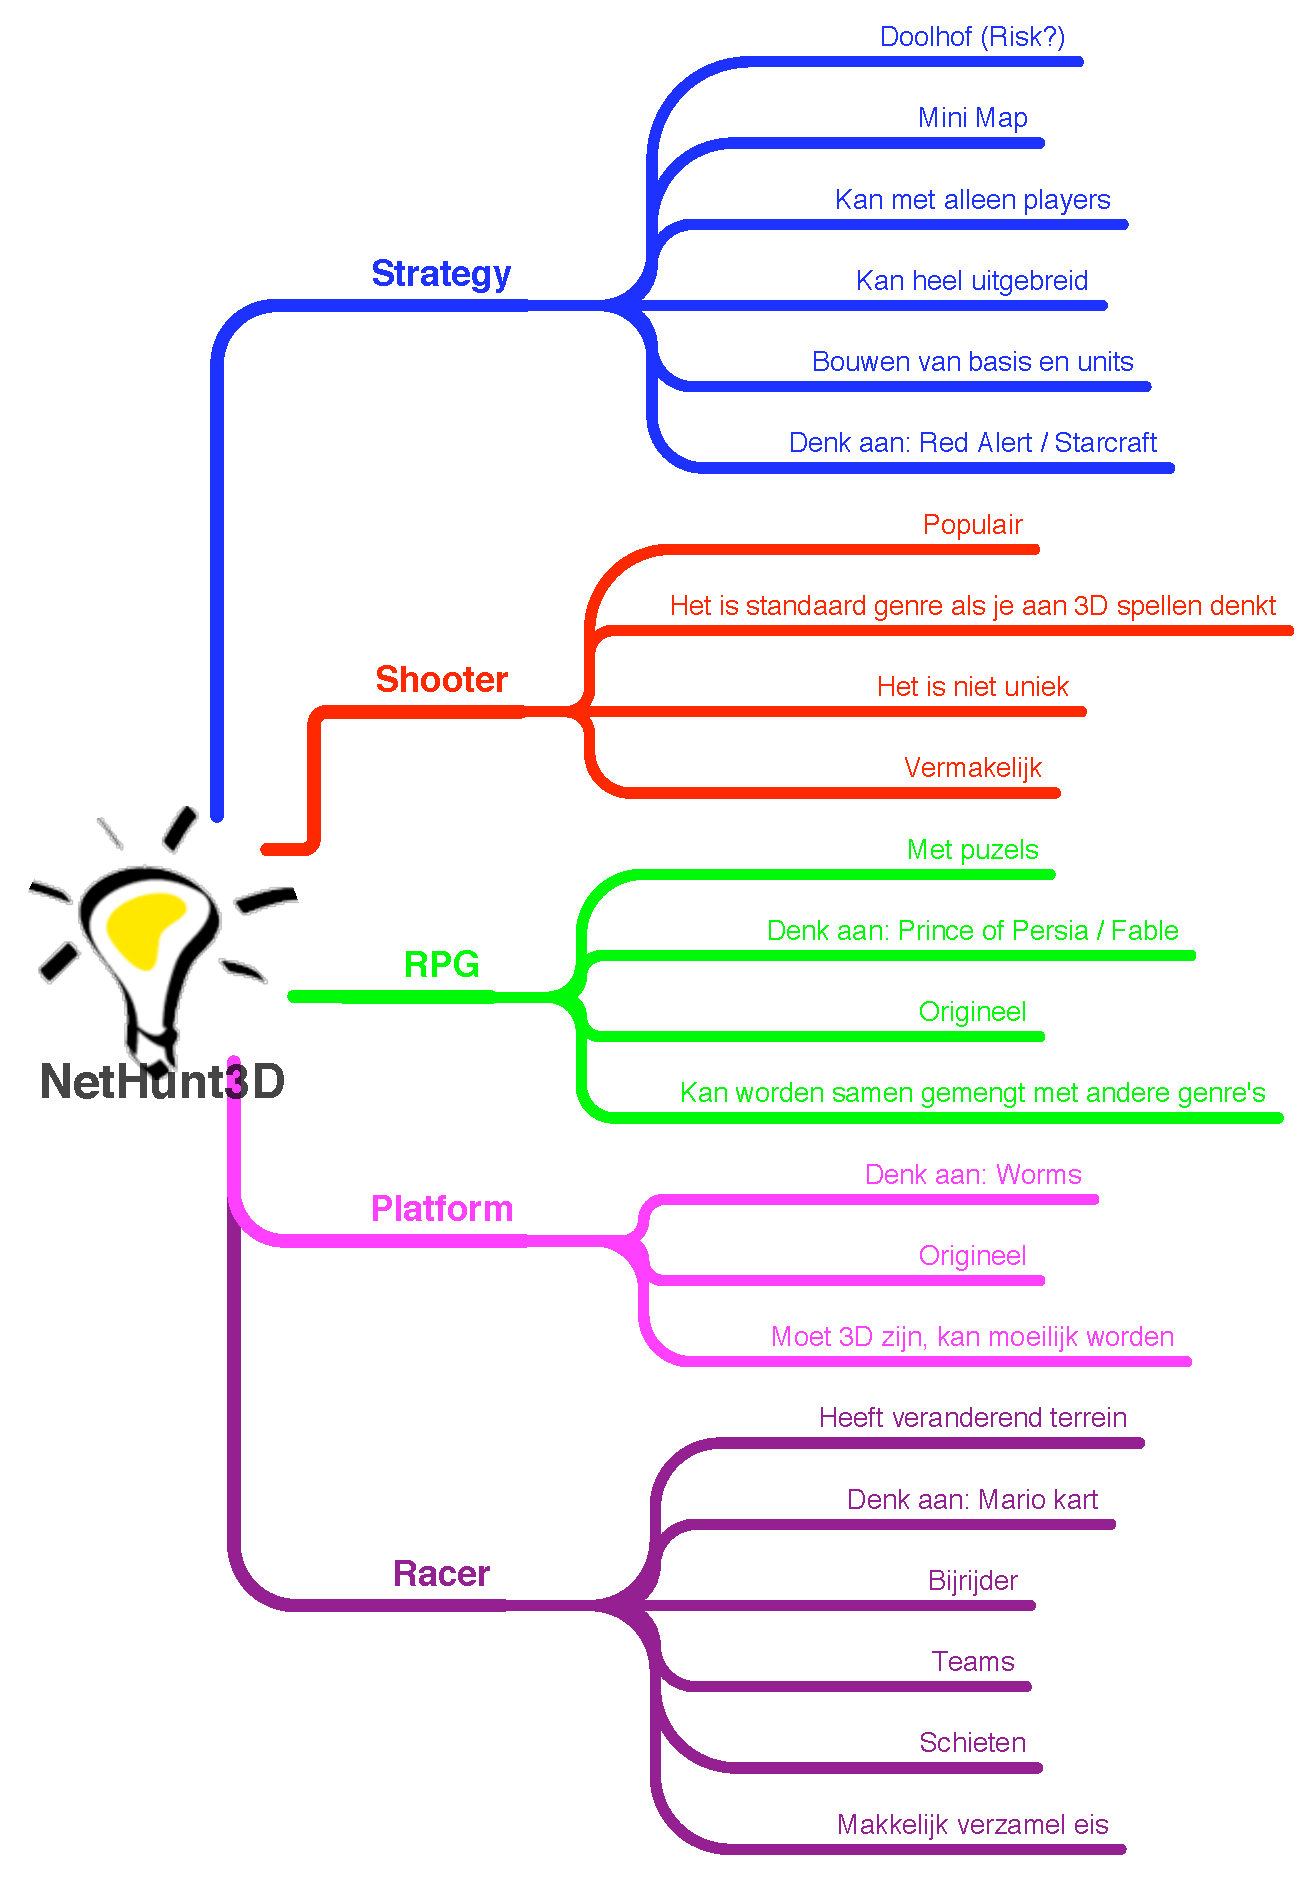
\includegraphics[width=9cm,height=14cm]{diagrams/mindmap1}
  \caption{The mind-map we came up with when choosing the genre} \label{fig:mindmap1}
\end{figure}

\begin{figure}[!ht]
  \centering
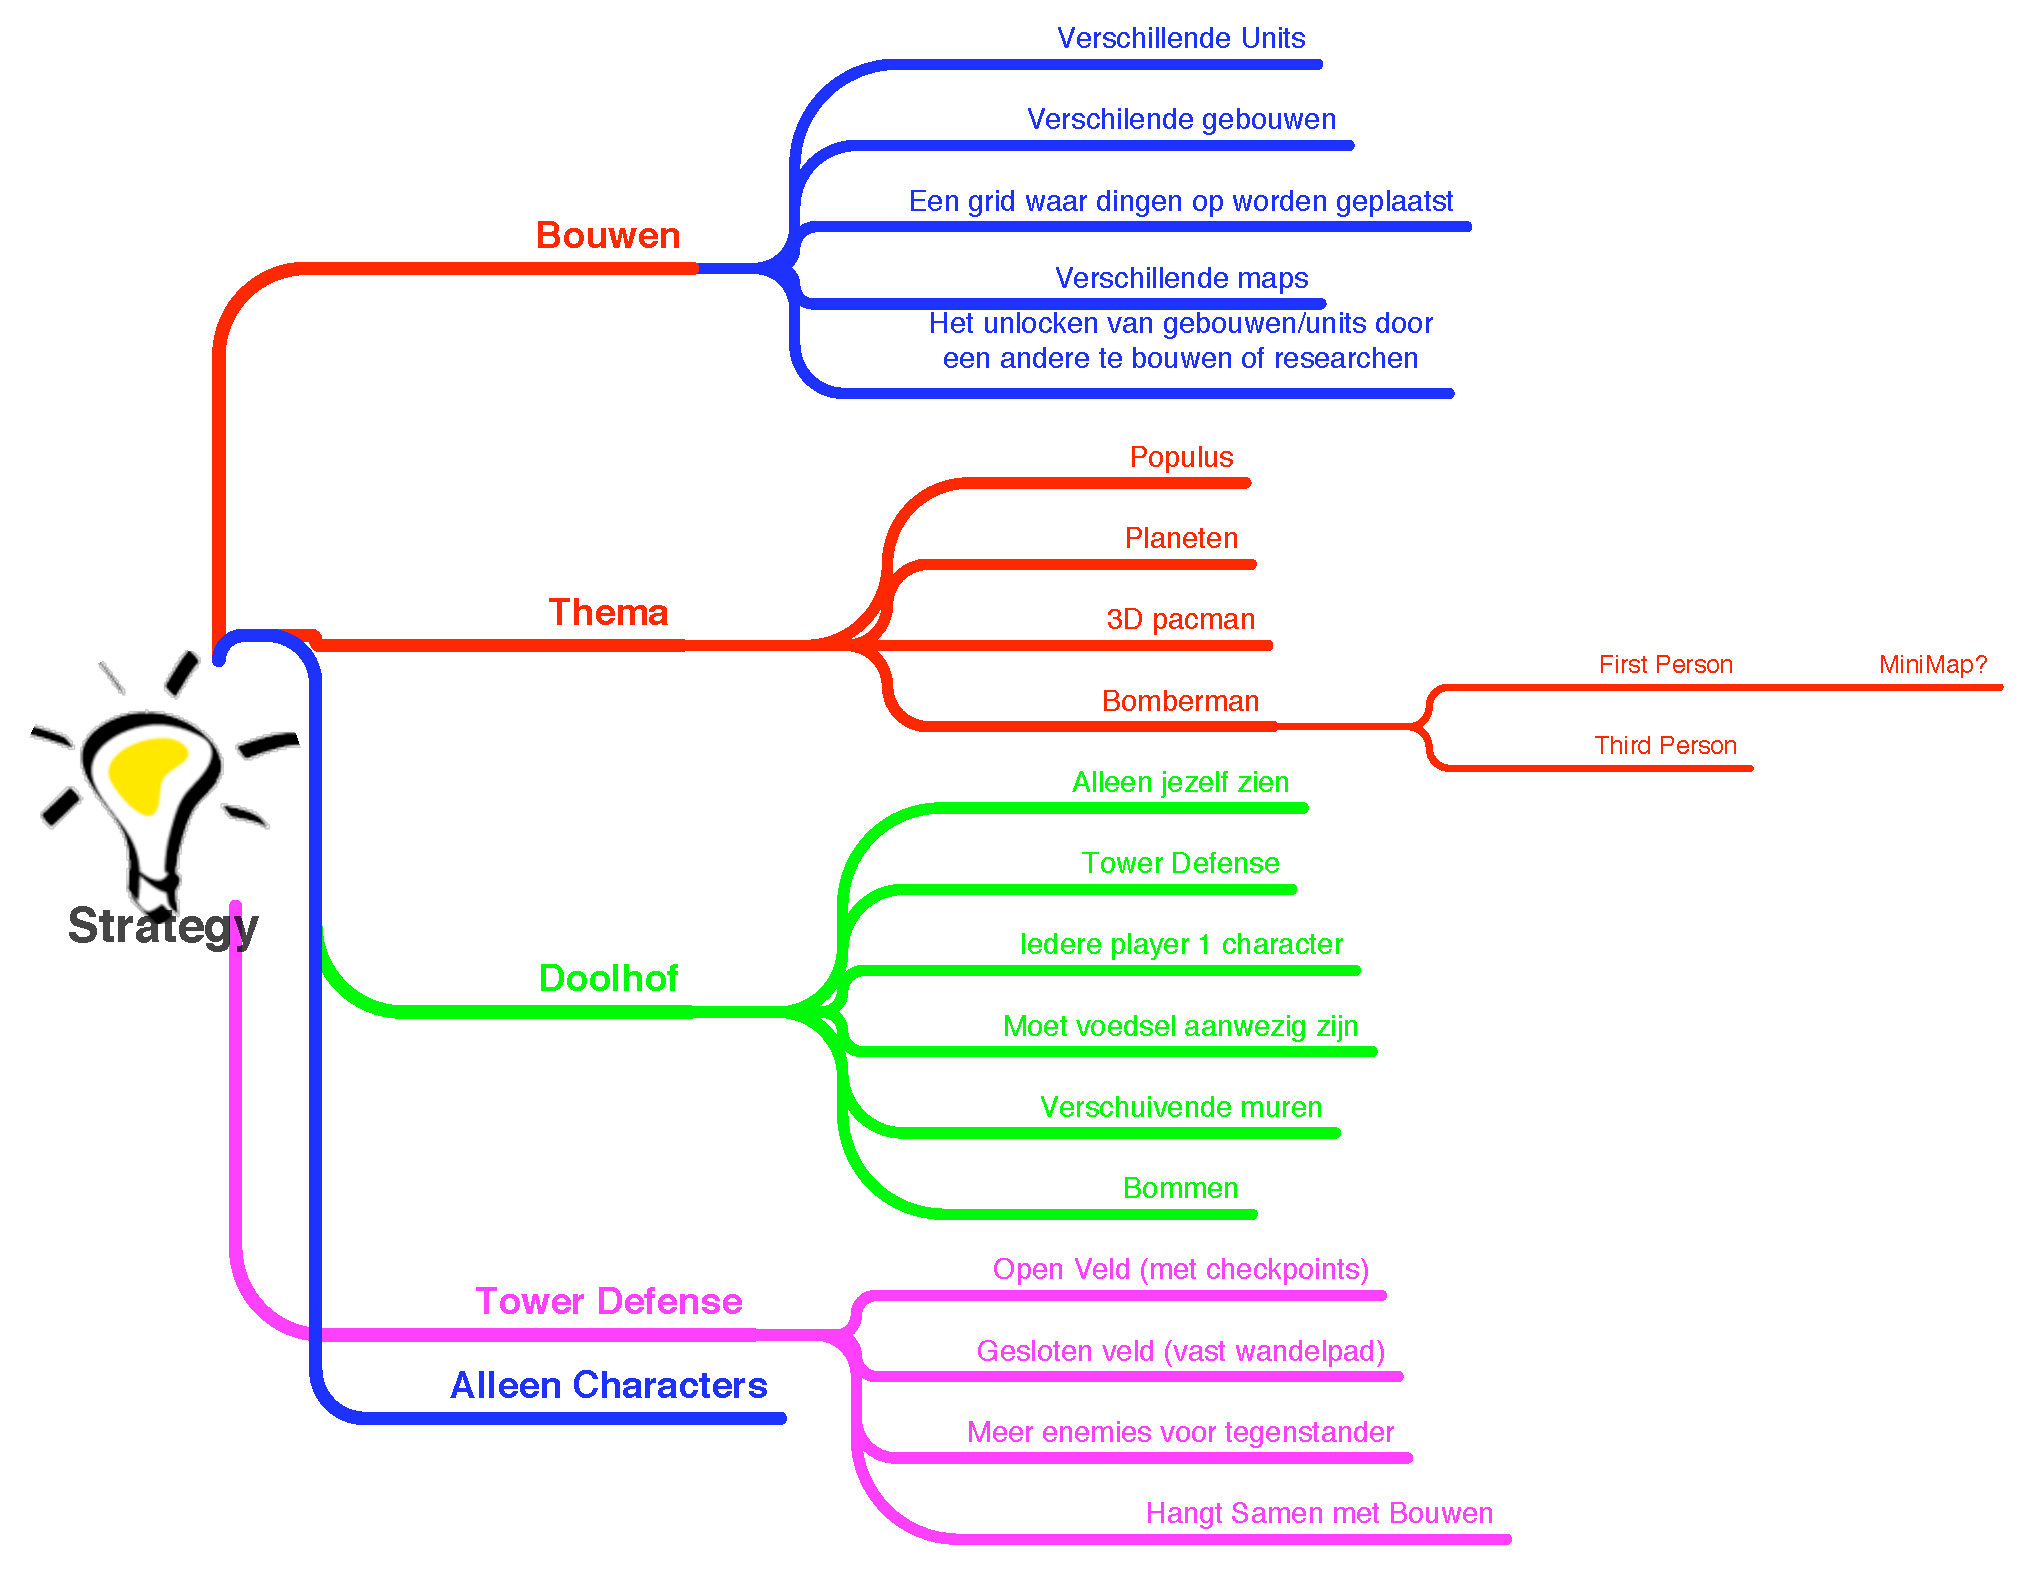
\includegraphics[width=11cm,height=10cm]{diagrams/mindmap2}
  \caption{The different styles of games are given in this mind-map. We eventually choose Bomberman} \label{fig:mindmap2}
\end{figure}


We decided on this formula because the basics are familiar, making for relatively straightforward implementation and because it has a popular and fast kind of gameplay with a low barrier to entry. Also, bombing and power-ups (see also: Table \ref{table:definitions}) allow us to give the game a unique look and feel.

\section{The features}

\subsection{Must have} % (fold)
\label{sec:must_have}
After our brainstorm session, we made a list of features that we want to implement, to make it a playable and fun game. These features are given in a MOSCoW list, giving features a higher to lower priority.

 \begin{itemize}
  \item Collision detection
  \item A map to play on
  \item Network functionality
  \item An interface
  \item Power-ups
 \end{itemize}
% section must_have (end)

\subsubsection{Reflection}
These features are all included in the game.

\subsection{Ought to have} % (fold)
\label{sec:ought_to_have}
The game ought to have these features to conform to reasonable expectations.

\begin{itemize}
  \item Weapons
  \item Audio
\end{itemize}
% section ought_have (end)

\subsubsection{Reflection}
We have not been very clear on what we meant by  `weapons'. Originally the idea behind this point was to have multiple kinds of weaponry, as many shooter games do. As the project progressed and our ideas about the desired gameplay solidified, it turned out that this would not contribute much to the gameplay, so it was scrapped. The program does have audio: there are sound effects and there is background music.

\subsection{Should have} % (fold)
\label{sec:should_have}
The game should have these features, they are feasible and improve it greatly.

\begin{itemize}
  \item Chatting
  \item Multiple maps
  \item Multiple avatar textures
\end{itemize}
% section should_have (end)

\subsubsection{Reflection}
There is support for chatting in the game, but we do not currently show chat messages on the screen. Chat  has been lowered in priority because the players are usually in the same room when playing our game anyway. We do have multiple maps support available for players (currently hard-coded). We do not have multiple avatar textures, which is the first serious point to be scrapped; there simply wasn't time to make or find them.

\subsection{Could have} % (fold)
\label{sec:could_have}
We might include these features, so we should design the game so that we can add them later.

\begin{itemize}
  \item A map editor
  \item Game rules (for mods)
  \item Different game modes
  \item Intro/victory/scenario movies
\end{itemize}
% section could_have (end)

\subsubsection{Reflection}
The game does not have a map editing function, although making maps takes little work once one knows the basics. The game does have an event engine, and therefore it supports the easy addition of new rules or the creation of new game modes in a way similar to that in which many shooter games do; people with some rudimentary programming knowledge can create new scripts, and put a reference to these rules in a map file. Any non-techsavvy player could then choose a map file when creating a game, and in this way have a completely customized game experience. The game does lack movies; it might have been better for us to put these in the `want to have'-section.

\subsection{Want to have} % (fold)
\label{sec:want_to_have}
If we have a lot of extra time, these are the features we want to add to the game.

\begin{itemize}
  \item Dynamics
  \item Physics
  \item No copyright material / Own copyright material
\end{itemize}
% section want_have (end)

\subsubsection{Reflection}
The textures we use are not copyright free. The sounds can be used for non-commercial use. We have researched the Open Dynamics library, but that would mean we would not have to make collision detection our selves, so that as scrapped. Integrating a better physics and dynamics engine would good for the gameplay of the game itself.

\section{Gameplay}
This description of the gameplay is based on the ``should have'' version of the game. Bomb3D is similar to the original Bomberman. Players, represented by avatars (see also: Table \ref{table:definitions}), spawn (see also: Table \ref{table:definitions}) in a level (see also: Table \ref{table:definitions}). They have a starting score, number of bombs and bomb range. They can move continuously (see also: Table \ref{table:definitions}) through a maze-like environment. Of course, players can not move through the walls of the maze, nor can they move through bombs, but they can move trough other avatars. There are two types of walls, walls which can be blown up by bombs, called ``Soft Walls''(see also: Table \ref{table:definitions}) and walls that cannot, the ``Hard Walls'' (see also: Table \ref{table:definitions}). The number of bombs denotes the amount of bombs which can be at most be set on the map at any given time. When a bomb of a player explodes, the player can place a new bomb.

Player interaction occurs mainly through ``bombing''; players can have a number of bombs at any one time, which they can leave anywhere in the maze. These bombs explode after a while, hitting anyone who is in range. The range of a bomb is the total range of the player. Players can gain extra bombs and bomb range by finding power-ups. These are located inside the soft walls of the games. When a certain wall is blown up, the power-up appears.\footnote{Not all walls contain power-ups, they are scattered randomly. Some may convey another bonus, if we can find the time to implement that.}

If players are hit, they are removed from the level and must wait for the next round. When only one player is left, that player has won the game. Each game has a time limit in which players can try to survive. When the clock has reached zero, the player with the most power-ups wins. The players' scores are kept throughout multiple games, showing their ranking in the ongoing competition.

\subsubsection{Reflection}
This has all been implemented as stated, with two exceptions: first, games are currently not time-limited, and second, scores are not kept throughout a `tournament' consisting of multiple games.

\section{Interface}
The players have a first person view (see also: Table \ref{table:definitions}) of the level, which takes up most of the screen. The other players' avatars and the level are shown in 3D, but the level is essentially 2D, that is, it can be described by a 2D map.

The players' number of bombs, their power and any special power-ups are all displayed in the game window, which also contains a minimap (see also: Table \ref{table:definitions}) showing the player's environment.

The graphical theme will be similar to the original Bomberman: cartoony and futuristic. This theme will not influence the game's implementation until much later in the project, however and the specifics are not set in stone. We expect our ideas about the theme to evolve as we continue working on the project.

Players use a combination of the mouse and keyboard to control their movements: they move the mouse to turn, click mouse buttons to perform basic actions (place bombs), use the arrow keys to move and sidestep and the other keyboard buttons for any special moves and actions which might be implemented.

\subsubsection{Reflection}
This has all been implemented as stated.

\section{GUI}

A number of important interface choices are described below.

\subsection{Menu Structure}
A list of menu types in our program:

\begin{itemize}
    \item Main menu
    \item Options menu
    \item Tournament searching menu
    \item New tournament creation menu
    \item Lobby menu
    \item Tournament overview screen
\end{itemize}

When a player starts the program, it shows the \emph{Main menu}, from which a player can enter the \emph{Tournament searching menu} or the \emph{Options menu}, or quit Bomb3D. In the \emph{Options menu}, a player can change the input and output settings of the game or return to the \emph{Main menu}. In the \emph{Tournament searching menu}, a player can see which other instances of the program have been found on the network and which tournaments have been started on the network. He or she can text-chat with other players, join an existing tournament or return to the \emph{Main menu}.

From the \emph{Tournament searching menu} a player can enter the \emph{New tournament creation menu}, where he or she can start a new game by choosing a level map file and tournament rules. After the player has clicked OK, the program shows the player a \emph{Lobby menu}, and it will broadcast the existence of his or her tournament to the other players. In a \emph{Lobby menu}, the player can see which other players have joined the same tournament, text-chat with other players, or start or cancel the tournament, the latter returning him or her to the \emph{Game searching menu}.

A tournament consists of several games. Between games, and at the start and end of a tournament, players see the \emph{Tournament overview screen}. This screen shows the current score (if any), and in it, the creator of the tournament can start the next round, remove players from the tournament or end the tournament prematurely.

\subsubsection{Reflection}
The graphical player interface supports most of these functions, though the menu structure is slightly different, and there is no way to chat with your peers over the network (though you can, of course, chat with them in real life, as you are probably in the same room)
\subsection{Visual Output}

\begin{figure}[!ht]
  \centering
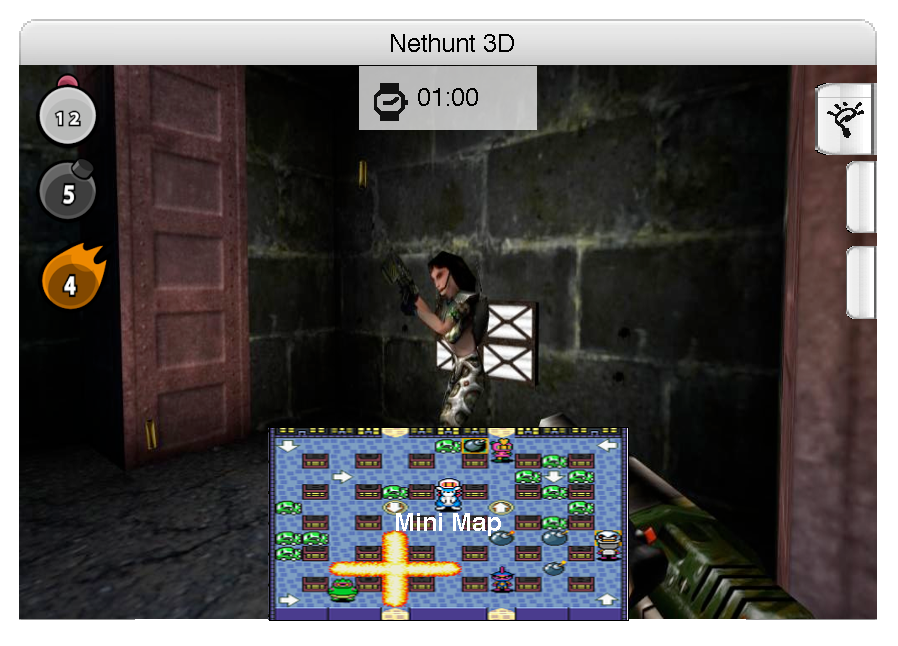
\includegraphics[width=\textwidth]{diagrams/interface}
  \caption{A mock-up of the interface} \label{fig:interface}
\end{figure}
\label{interface}

This is the way in which our visual output to the player will be organized, as illustrated in Figure~\ref{fig:interface}.

The program can be run in a window or fullscreen, with fullscreen being the default. During a game, most of the screen will be taken up a by a 3D visual depiction of the player's in-game surroundings.

In the top left corner of the screen, along the left side, will be the player's score, the maximum number of bombs they can create and the reach of their bombs' explosions. In the top right corner of the screen, along the right side, will be three slots which can be filled by the power-ups which the player has collected and has yet to use. Only three power-ups can be stored in this way at any one time.

The clock is located at the top of the screen, which displays the time left to play in the current game (if applicable).

In the lower center of the screen, at its bottom edge, will be a display of the map of the level, with moving 2D sprites giving a lot of information about the action which is taking place, facilitating strategic decision making. At the touch of a button, the minimap is enlarged to being about half as high and wide as the screen, or reduced to being about a quarter of the screen's height and length in size.

The chat function will display an input field an others' text in the bottom of the screen.

\subsubsection{Reflection}
There is no way to change the display mode from windowed to fullscreen in-game. For testing purposes, we changed the default to windowed mode. There is also no clock, as games are not timed. The minimap cannot be enlarged; it is large enough to see everything which is going on in the level, and enlarging to would block a lot of the player's vision. There is no chat functionality.

The interface is a part of the game which could have been improved a lot with little extra time; most of the things it lacks are simple to implement. Unfortunately, we had other things to finish first.


\subsection{Input}

While in a game, the player can use the mouse to look around. There will be a default assignment of mouse buttons and keys to actions, which can be changed by the player.

The default input configuration is as follows. The player moves around using the $W$, $A$, $S$ and $D$ keys. $W$ moves the avatar forward, $S$ moves him backward, and $A$/$D$ is used to move sideways. Bombs are dropped using the left mouse button. The numeric keys are used to activate the corresponding power-up. The arrow keys will be used for basic navigation through the program's menus, which can also be controlled with the cursor.

List with input keys:
 \begin{itemize}
    \item $W$: Move forward.
    \item $S$: Move backward.
    \item $A$: Step sideways (left).
    \item $D$: Step sideways (right).
    \item $1$: Activate power-up 1.
    \item $2$: Activate power-up 2.
    \item $3$: Activate power-up 3.
    \item $M$: Toggles the size of the minimap.
    \item $TAB$: Toggles the chat window (when implemented).
    \item $Mouse Movement$: Look around.
    \item $Left Mouse Button$: Drop Bomb.
 \end{itemize}

\subsubsection{Reflection}
There is an ini-file containing the key mappings, though there is currently no way to change it.

\section{Winning the game}
The main goal of the game (varying slightly between game modes) is being the last man standing in the most games.

We might include the option to play the game in different modes, in which the objectives vary, if we have time. Inspiration on that matter can easily be drawn from so called ``shooter'' games and these modes may include:

\begin{itemize}
  \item Deathmatch, in which the objective is doing as much bombing of others as possible within limited time or within a limited number of respawns.

  \item Capture the flag, in which the players are divided into teams and the objective is to steal the other team's ``flag''-power-up from their base and run back with it to your own base.

  \item Greed, in which the player who gathers most power-ups wins.
\end{itemize}

\subsubsection{Reflection}
This works as stated. No extra game modes have been implemented, though can easily be scripted.

\subsection{Technological}

We will use a star-network for communication between the players. For the graphics we will use Python and OpenGL with the PyOpenGL package for binding them. We will also use the PyGame library for some auxiliary functions, though we will still have to do the main graphics programming ourselves, as PyGame only helps with 2D graphics.

The program will consist of several components: a main component which handles the graphics and the game state, one for the network and one to handle player input.

\subsubsection{Reflection}
Very shortly before delivering this document for the first time, we changed the network type from ``token-ring'' to ``star'', to reflect our plans at that time. Unfortunately, these plans turned out to be too ambitious. We turned to using a token-ring network anyway when the implementation phase rolled around. The PyGame library turned out to be useful, though quirky. It turned out, for example, that input reading under PyGame could not be executed in another thread than screen updating.

As explained in the design document, our program is more complex, and has more components, than stated here. Significantly, graphics and game state handling (engine) have been separated. This specification document gives only a vague, preliminary sketch, so that was to be expected.

% chapter specification (end) 